%%
%% PollingLab (c) 2021-22 Christopher A. Bohn
%%

%%
%% (c) 2021 Christopher A. Bohn
%%

\documentclass[12pt]{article}

\usepackage{fullpage}
\usepackage{fancyhdr}
\usepackage[procnames]{listings}
\usepackage{hyperref}
\usepackage{textcomp}
\usepackage{bold-extra}
\usepackage[dvipsnames]{xcolor}
\usepackage{etoolbox}


% Customize the semester (or quarter) and the course number

\newcommand{\courseterm}{Spring 2022}
\newcommand{\coursenumber}{CSCE 231}

% Customize how a typical lab will be managed;
% you can always use \renewcommand for one-offs

\newcommand{\runtimeenvironment}{your account on the \textit{csce.unl.edu} Linux server}
\newcommand{\filesource}{Canvas or {\footnotesize$\sim$}cse231 on \textit{csce.unl.edu}}
\newcommand{\filesubmission}{Canvas}

% These are placeholder commands and will be renewed in each lab

\newcommand{\labnumber}{}
\newcommand{\labname}{Lab \labnumber\ Assignment}
\newcommand{\shortlabname}{}
\newcommand{\duedate}{}

% Individual or team effort

\newcommand{\individualeffort}{This is an individual-effort project. You may discuss concepts and syntax with other students, but you may discuss solutions only with the professor and the TAs. Sharing code with or copying code from another student or the internet is prohibited.}
\newcommand{\teameffort}{This is a team-effort project. You may discuss concepts and syntax with other students, but you may discuss solutions only with your assigned partner(s), the professor, and the TAs. Sharing code with or copying code from a student who is not on your team, or from the internet, is prohibited.}
\newcommand{\freecollaboration}{In addition to the professor and the TAs, you may freely seek help on this assignment from other students.}
\newcommand{\collaborationrules}{}

% Do you care about software engineering?

\providebool{allowspaghetticode}

\setbool{allowspaghetticode}{false}

\newcommand{\softwareengineeringfrontmatter}{
    \ifboolexpe{not bool{allowspaghetticode}}{
        \section*{No Spaghetti Code Allowed}
        In the interest of keeping your code readable, you may \textit{not} use
        any \lstinline{goto} statements, nor may you use any \lstinline{break}
        statements to exit from a loop, nor may you have any functions
        \lstinline{return} from within a loop.
    }{}
}

\newcommand{\spaghetticodepenalties}[1]{
    \ifboolexpe{not bool{allowspaghetticode}}{
        \penaltyitem{1}{for each \lstinline{goto} statement, \lstinline{break}
            statement used to exit from a loop, or \lstinline{return} statement
            that occurs within a loop.}
    }{}
}

% You shouldn't need to customize these,
% but you can if you like

\lstset{language=C, tabsize=4, upquote=true, basicstyle=\ttfamily}
\newcommand{\function}[1]{\textbf{\lstinline{#1}}}
\setlength{\headsep}{0.7cm}
\hypersetup{colorlinks=true}

\newcommand{\startdocument}{
    \pagestyle{fancy}
    \fancyhf{}
    \lhead{\coursenumber}
    \chead{\ Lab \labnumber: \labname}
    \rhead{\courseterm}
    \cfoot{\shortlabname-\thepage}

	\begin{document}
	\title{\ Lab \labnumber}
	\author{\labname}
	\date{Due: \duedate}
	\maketitle

    \textit{\collaborationrules}
}

\newcommand{\rubricitem}[2]{\item[\underline{\hspace{1cm}} +#1] #2}
\newcommand{\bonusitem}[2]{\item[\underline{\hspace{1cm}} Bonus +#1] #2}
\newcommand{\penaltyitem}[2]{\item[\underline{\hspace{1cm}} -#1] #2}

\usepackage{enumitem}
\usepackage{graphicx}
\usepackage{addfont}
\addfont{OT1}{d7seg}{\dviiseg}
% \addfont{OT1}{deseg}{\deseg}
\usepackage{subfig}
% \usepackage{wrapfig}
\usepackage{multicol}
% \usepackage{caption}
% \captionsetup{width=.8\linewidth}

% \lstset{language=c, numbers=left, showstringspaces=false,
%     moredelim = [s][\ttfamily]{/*}{*/} % I shouldn't need this parameter!
%     }



\renewcommand{\labnumber}{8}
\renewcommand{\labname}{Using Polling with Memory-Mapped Input/Output}
\renewcommand{\shortlabname}{memory-mapped i/o -- pollinglab}
\renewcommand{\collaborationrules}{\individualeffort}
%\renewcommand{\duedate}{soon}
\renewcommand{\duedate}{Week of April 11, Before the start of your lab section}
\newcommand{\nano}{Arduino Nano}
\renewcommand{\runtimeenvironment}{your \nano-based class hardware kit}

\startdocument

In this assignment, you will write functions to use the input and output
devices on \runtimeenvironment. You will then use those functions to implement
the ability to build a number, similar to entering a value on a calculator,
using polling.

\begin{figure}[h]
    \centering
    \includegraphics[width=10cm]{AreWeThereYet}
    \caption{Polling. \tiny Image by 20th Century Fox Television}
\end{figure}

The instructions are written assuming you will edit the code in the Arduino IDE
and run it on \runtimeenvironment, constructed according to the pre-lab
instructions. If you wish, you may edit the code in a different environment;
however, our ability to provide support for problems with other IDEs is limited.

Please familiarize yourself with the entire assignment before beginning.
Section~\ref{sec:FunctionalSpecification} has the functional specification of
the system you will develop. Section~\ref{sec:Constraints} describes
implementation constraints. Section~\ref{sec:DemonstrationMode} guides you in
implementing the first portion of the system, and
Section~\ref{sec:BuildingMode} offers suggestions in implementing the second
portion of the system.

\section*{Learning Objectives}

After successful completion of this assignment, students will be able to:
\begin{itemize}
\item Use memory-mapped I/O to obtain inputs from peripheral devices
\item Use memory-mapped I/O to send outputs to peripheral devices
\item Poll an input to determine when it has taken on a value of interest
\item Scan a matrix keypad
\item Use the Serial-Parallel Interface (SPI) protocol
\item Display a value or a message on a collection of 7-segment displays
\end{itemize}

\subsection*{Continuing Forward}

We will use the hardware kit for the remaining labs. In the labs after this one,
you will not be required to use the memory-mapped I/O registers (but you may!);
however, we will assume that you know how to scan a matrix keypad, and that you
can build and display a value from keypad inputs.

\section*{During Lab Time}

During your lab period, the TAs will provide a refresher on bitmasks, both to
read inputs and to use the read-modify-write pattern for outputs. They will also
demonstrate creating the bit patterns that you will use for the 7-segment
display module by guiding students through a discussion and discovery of the
bit pattern for the numeral {\dviiseg 2}. During the remaining time, the TAs
will be available to answer questions.

\softwareengineeringfrontmatter

\section{Scenario}

Archie walks up to you, along with Herb Bee from Eclectic Electronics. Herb is
holding a tangled mess of electronics. Archie explains, ``Herb here has
developed a prototype of a device that he thinks will be useful for our
physical security needs, as well as a few other applications around here. He
calls it the \textit{Cow Pi}.''

You look at the device in Herb's hands and see the \nano\ central to the circuit. ``Isn't \textit{-Pi} typically used as a suffix for circuits that use a Raspberry Pi instead of an Arduino?''

Herb replies, ``Typically, yes, but \textit{Cowduino} isn't very punny, is it?''

Archie chimes in, ``Maybe with the right emphasis: \textit{Cow-DOO-ino}.''

``That's kind of subtle, don't you think? How will people know to put the
emPHAsis on that sylLAble?''

``I think we're getting off topic here,'' you point out. ``How can I help?''

``Oh, right,'' Herb says, ``We'd like you to kick its proverbial tires. Let's
start off with something simple, like a number builder tool.''

\section{Number Builder Specification} \label{sec:FunctionalSpecification}

\begin{enumerate}
\item The tool shall have two modes, \textit{demonstration mode} and
    \textit{builder mode}. The \textbf{left switch} controls the mode.
\item The tool shall have two number bases, \textit{decimal} and
    \textit{hexadecimal}. The \textbf{right switch} controls the number base.
\item \label{spec:decimalExplained} When the \textbf{right switch} is toggled
    to the left, the number builder will use the decimal number base. When the
    user presses a button on the \textbf{matrix keypad} with a decimal numeral
    (\textit{0-9}) then the number builder shall take the appropriate action as
    specified in requirement \ref{spec:demonstrationKeyPress} or
    \ref{spec:BuildingValue}. Any other buttons on the keypad shall be ignored.
\item \label{spec:hexadecimalExplained} When the \textbf{right switch} is
    toggled to the right, the number builder will use the hexadecimal number
    base. When the user presses a button on the \textbf{matrix keypad} then the
    number builder shall take the appropriate action as specified in
    requirement \ref{spec:demonstrationKeyPress} or \ref{spec:BuildingValue}.
    Buttons with decimal numerals (\textit{0-9}) or alphabetic letters
    (\textit{A-D}) shall be interpreted as having the corresponding hexadecimal
    numeral; the button with the octothorp (\#) shall be interpreted as having
    the hexadecimal numeral \textit{E}; and the button with the asterisk (*)
    shall be interpreted as having the hexadecimal numeral \textit{F}.
\item Initially, no digits on the \textbf{7-segment display module} shall have
    any of their segments illuminated.
\item When the \textbf{left switch} is toggled to the left, the number builder
    is in demonstration mode. When the number builder is in demonstration mode:
    \begin{enumerate}
    \item \label{spec:illuminateLED} Whenever the user presses a button on the
        \textbf{matrix keypad}, the \textbf{external LED} shall illuminate for
        approximately one-half of a second.
    \item The \textbf{external LED} shall not illuminate except as specified in
        requirement~\ref{spec:illuminateLED}.
    \item \label{spec:demonstrationKeyPress} Whenever the user presses a button
        on the \textbf{matrix keypad}, the corresponding numeral shall be
        displayed in the least-significant digit position of the
        \textbf{7-segment display module}, replacing any numeral previously
        displayed. The numeral displayed shall follow the interpretations
        specified in requirements \ref{spec:decimalExplained} and
        \ref{spec:hexadecimalExplained}.
    \item If the user toggles the \textbf{right switch} (\textit{i.e.}, changes
        the number base) while in demonstration mode, then the numeral being
        displayed shall continue to be displayed even if it is an invalid
        numeral in the new number base. The system shall, however, respect the
        new number base for future keypresses.
    \item While the system is in demonstration mode, here are no requirements
        nor restrictions with respect to printing to the Serial Monitor.
    \item Whenever the user presses the \textbf{right pushbutton} while the
        system is in demonstration mode, the \textbf{7-segment display module}
        shall be cleared: no segments shall be illuminated.
    \end{enumerate}
\item \label{spec:ConversionMode} When the \textbf{left switch} is toggled to
    the right, the number builder is in builder mode. When the number builder
    is in builder mode:
    \begin{enumerate}
    \item \label{spec:BuildingValue} Whenever the user presses a button on the
        \textbf{matrix keypad}, the corresponding numeral shall be displayed in
        the least-significant position of the \textbf{7-segment display
        module}, and any digits already displayed shall increase in
        significance by one order of magnitude. For example, if {\dviiseg 234}
        is displayed and the user presses \texttt{5} then {\dviiseg 2345} shall
        be displayed. The numeral displayed shall follow the interpretations
        specified in requirements \ref{spec:decimalExplained} and
        \ref{spec:hexadecimalExplained}.
        \begin{enumerate}
        \item There shall be no noticeable lag in updating the display.
        \item \label{spec:printValueToConsole} The new value shall be printed
            to the Serial Monitor in decimal or hexadecimal, depending on the
            system's current number base.
        \end{enumerate}
    \item Whenever the user presses the \textbf{left pushbutton}, the value
        being displayed shall be negated.
        \begin{enumerate}
        \item In the decimal number base, the presence or absence of negative
            sign shall indicate whether or not a value is negative
        \item In the hexadecimal number base, 32-bit two's complement shall be
            used.
        \end{enumerate}
    \item ``0x'' shall not be displayed as part of a hexadecimal value.
    \item A positive sign shall not be displayed as part of a positive value.
    \item If a negative decimal value is displayed, the negative sign shall
        be displayed immediately to the left of the most-significant digit
        being displayed. For example, {\dviiseg-456} is correctly
        displayed, but {\dviiseg -    456} is not correctly displayed.
    \item Leading 0s may be displayed but are discouraged. For example,
        {\dviiseg 782} is preferred, but {\dviiseg 00000782} is allowed.
    \item In no case shall the tool allow the user to input a value too
        great to be displayed on the \textbf{7-segment display module}. If
        the user attempts to enter a value greater than $0x7FFF,FFFF$ in
        hexadecimal, less than $0x8000,0000$ in hexadecimal, greater than
        $99,999,999$ in decimal, or less than $-9,999,999$ in decimal, then the
        \textbf{7-segment display module} shall display {\dviiseg too big}.
        \begin{itemize}
        \item \textit{n.b.}, in a hexadecimal 32-bit negative integer, an
            \texttt{F} in the most-significant hex-digit might only be a sign
            extension; in this scenario, if the user inputs another hex-digit
            then it is still a valid number because it would not be less than
            $0x8000,0000$. \\ \\
            For example, adding another digit to the 32-bit integer
            $0xF865,4321$ would \textit{not} produce a too-great value because
            the 36-bit integer $0xF,8654,3210 = -2,041,302,512_{10}$, and the
            32-bit integer $0x8654,3210 = -2,041,302,512_{10}$. Because
            $0x8000,0000 = -2,147,483,648_{10} \leq -2,041,302,512_{10}$, adding
            the \texttt{0} digit did not produce a ``too big'' value. \\ \\
            On the other hand, adding another digit to the 32-bit integer
            $0xF765,4321$ \textit{would} produce a too-great value because the
            36-bit integer $0xF,7654,3210 = -2,309,737,968_{10}$, but the 32-bit
            integer $0x8654,3210 = 1,985,229,328_{10}$. Because
            $0x8000,0000 = -2,147,483,648_{10} > -2,309,737,968_{10}$, adding
            the \texttt{0} digit did produce a ``too big'' value.
        \end{itemize}
    \item Except as specified in requirement \ref{spec:printValueToConsole},
        nothing shall be printed on the Serial Montior when the system is in
        building mode.
    \item If the user toggles the \textbf{right switch} (\textit{i.e.}, changes
        the number base) while in builder mode: if the number being built is 0
        then the system shall seamlessly transition between number bases; if
        the number being built is not 0 then the system's behavior is
        unspecified.
    \item Whenever the user presses the \textbf{right pushbutton} while the
        system is in builder mode, the number being built shall reset to 0, and
        the \textbf{7-segment display module} shall be cleared, \textit{except}
        that the least-significant digit shall display a 0 (this being the new
        number being built).
    \end{enumerate}
\item If the user changes modes (\textit{i.e.}, toggles the \textbf{left
    switch}) then the following behavior is recommended but not required:
    \begin{enumerate}
    \item When changing from demonstration mode to builder mode, the numeral
        being displayed (if any) may become the most-significant digit of the
        number to be built.
    \item When changing from builder mode to demonstration mode, the numerals
        to the left of the least-significant digit (if any) may continue to be
        displayed without significance.
    \end{enumerate}
\item When the user presses a button for less than approximately one-half of a
    second, regardless of whether it is one of the \textbf{pushbuttons} or a
    button on the \textbf{matrix keypad}, it shall be treated as a single
    button press.
\end{enumerate}

\section{Constraints}\label{sec:Constraints}

All input and output must be accomplished using the memory-mapped I/O
registers. You may use any constants, arrays, structs, typedefs, or macros
present in the \textit{cowpi.h} header file provided as part of this
assignment. You may use any code that you write yourself. You may use any
features that are part of the C standard if they are supported by the
compiler. Except as noted below, you may \textit{not} use any libraries,
functions, macros, types, or constants that are part of the Arduino
core\footnote{\url{https://www.arduino.cc/reference/en/}} (unless they are
also part of the C standard), nor AVR-specific functions, macros, types, or
constants of avr-libc\footnote{\url{https://www.nongnu.org/avr-libc/user-manual/index.html}}.

You \textit{may} use the
\function{millis()}\footnote{\url{https://www.arduino.cc/reference/en/language/functions/time/millis/}}
function to measure the passage of time, and you \textit{may} use the
\function{Serial.begin()}\footnote{\url{https://www.arduino.cc/reference/en/language/functions/communication/serial/begin/}},
\function{Serial.print()}\footnote{\url{https://www.arduino.cc/reference/en/language/functions/communication/serial/print/}}, and
\function{Serial.println()}\footnote{\url{https://www.arduino.cc/reference/en/language/functions/communication/serial/println/}} functions for debugging
and for implementing requirement \ref{spec:printValueToConsole}. \textit{Be
sure to remove \function{print()} and \function{println()} calls that are used
only for debugging before turning in your code for grading.}

(A quick note on using \function{print()} and \function{println()} for
debugging: if you print too much, the UART buffer may fill, making it
difficult to upload a new program to the \nano. If you have an upload
failure in this situation, the simplest fix in this case is to unplug the
\nano, plug it back in, and re-attempt the upload.) (Another quick note on
using \function{print()} and \function{println()}: please read these functions'
documentation to understand what the functions can -- and can't -- do.)

\section{Implementing Demonstration Mode} \label{sec:DemonstrationMode}

You will use ``demonstration mode'' to configure your \nano\ to use the
memory-mapped input/output controls and peripheral devices.

\subsection{Simple Input/Output}

The ATmega328P microcontroller\footnote{\url{http://ww1.microchip.com/downloads/en/DeviceDoc/Atmel-7810-Automotive-Microcontrollers-ATmega328P_Datasheet.pdf}}
on the \nano\ has three input/output ports accessible by external pins. Each
port has three registers, the PIN input register, the PORT output register, and
the DDR data direction register used to set each pin as input or output. Each
pin is individually controlled by a particular bit in the port registers.
Figure~\ref{fig:IoPortRegisters} shows these nine registers and their
corresponding addresses.
You do not need to configure the pins for input or output; the
\function{cowpi_setup} macro provided in \textit{cowpi.h} takes care of all
necessary configuration.

\begin{figure}
    \centering
    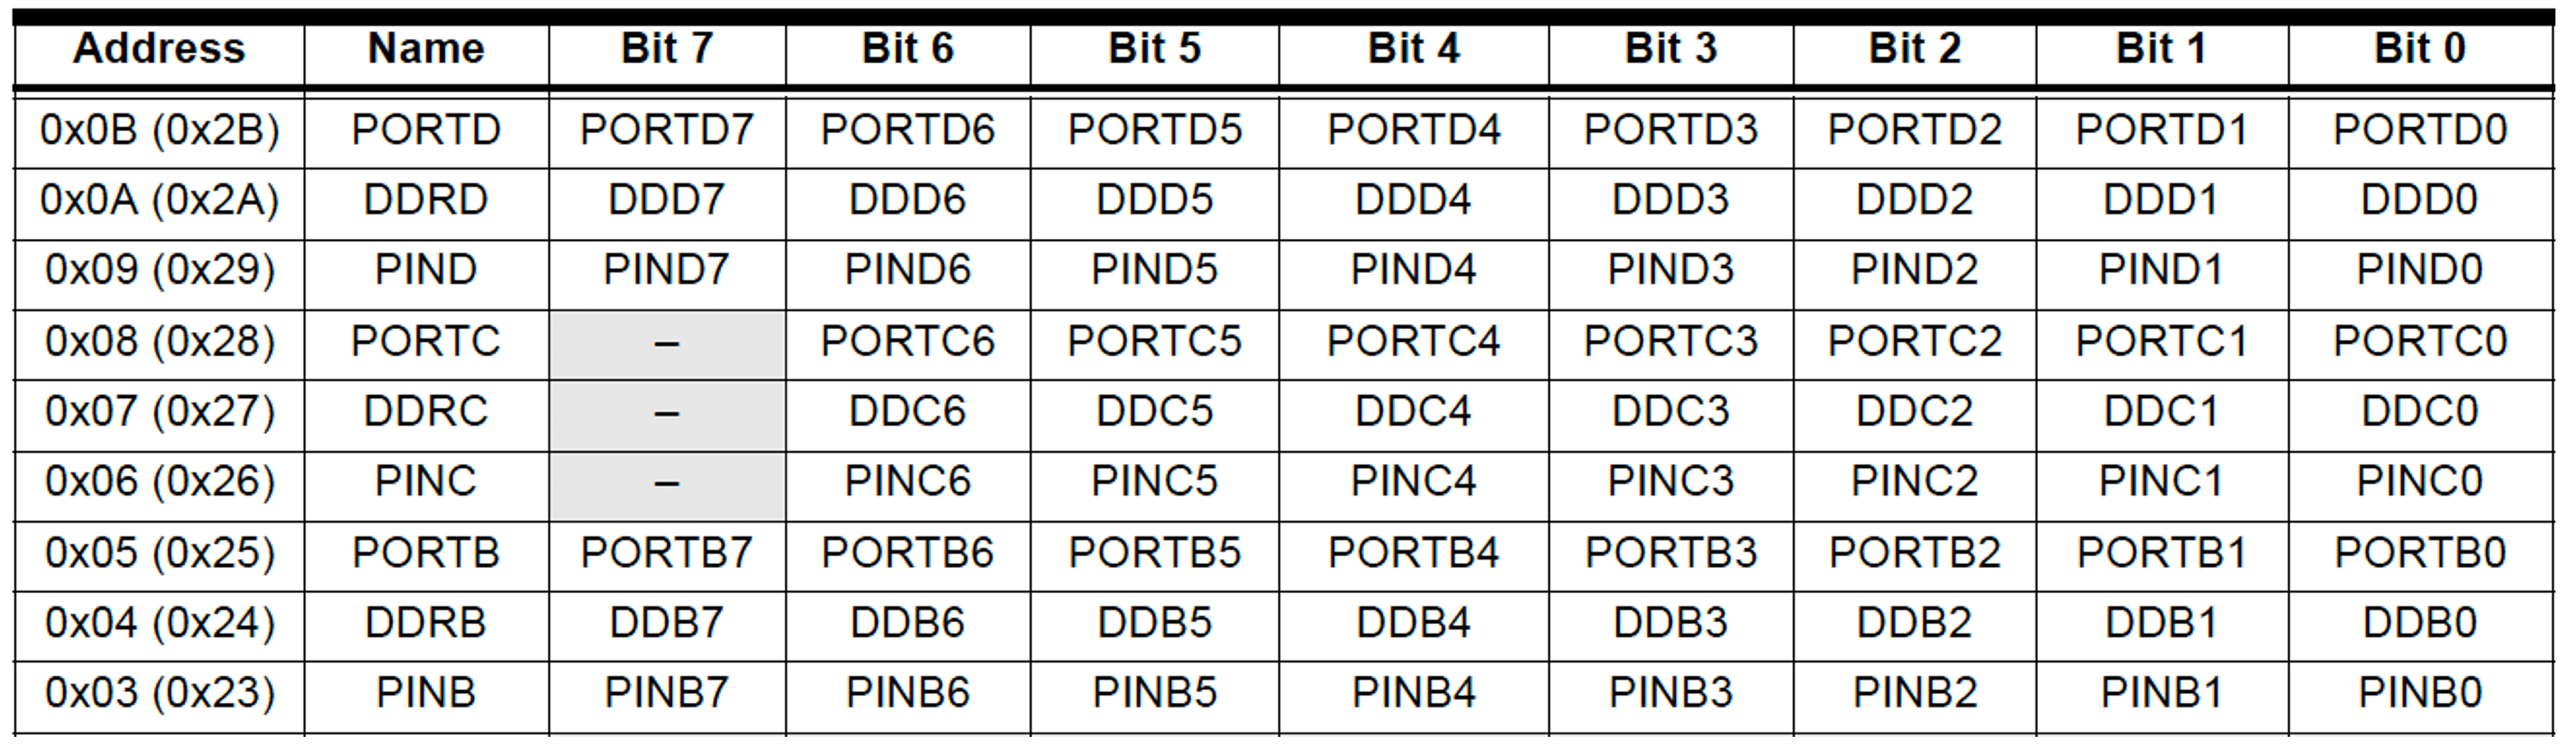
\includegraphics[width=15cm]{IoPortRegisters}
    \caption{ATmega328P I/O port registers. Each register's I/O address and
        memory address (in parentheses) are provided. \tiny Cropped from
        ATmega382P Data Sheet, §30 \label{fig:IoPortRegisters}}
\end{figure}

\begin{figure}[h]
    \centering
    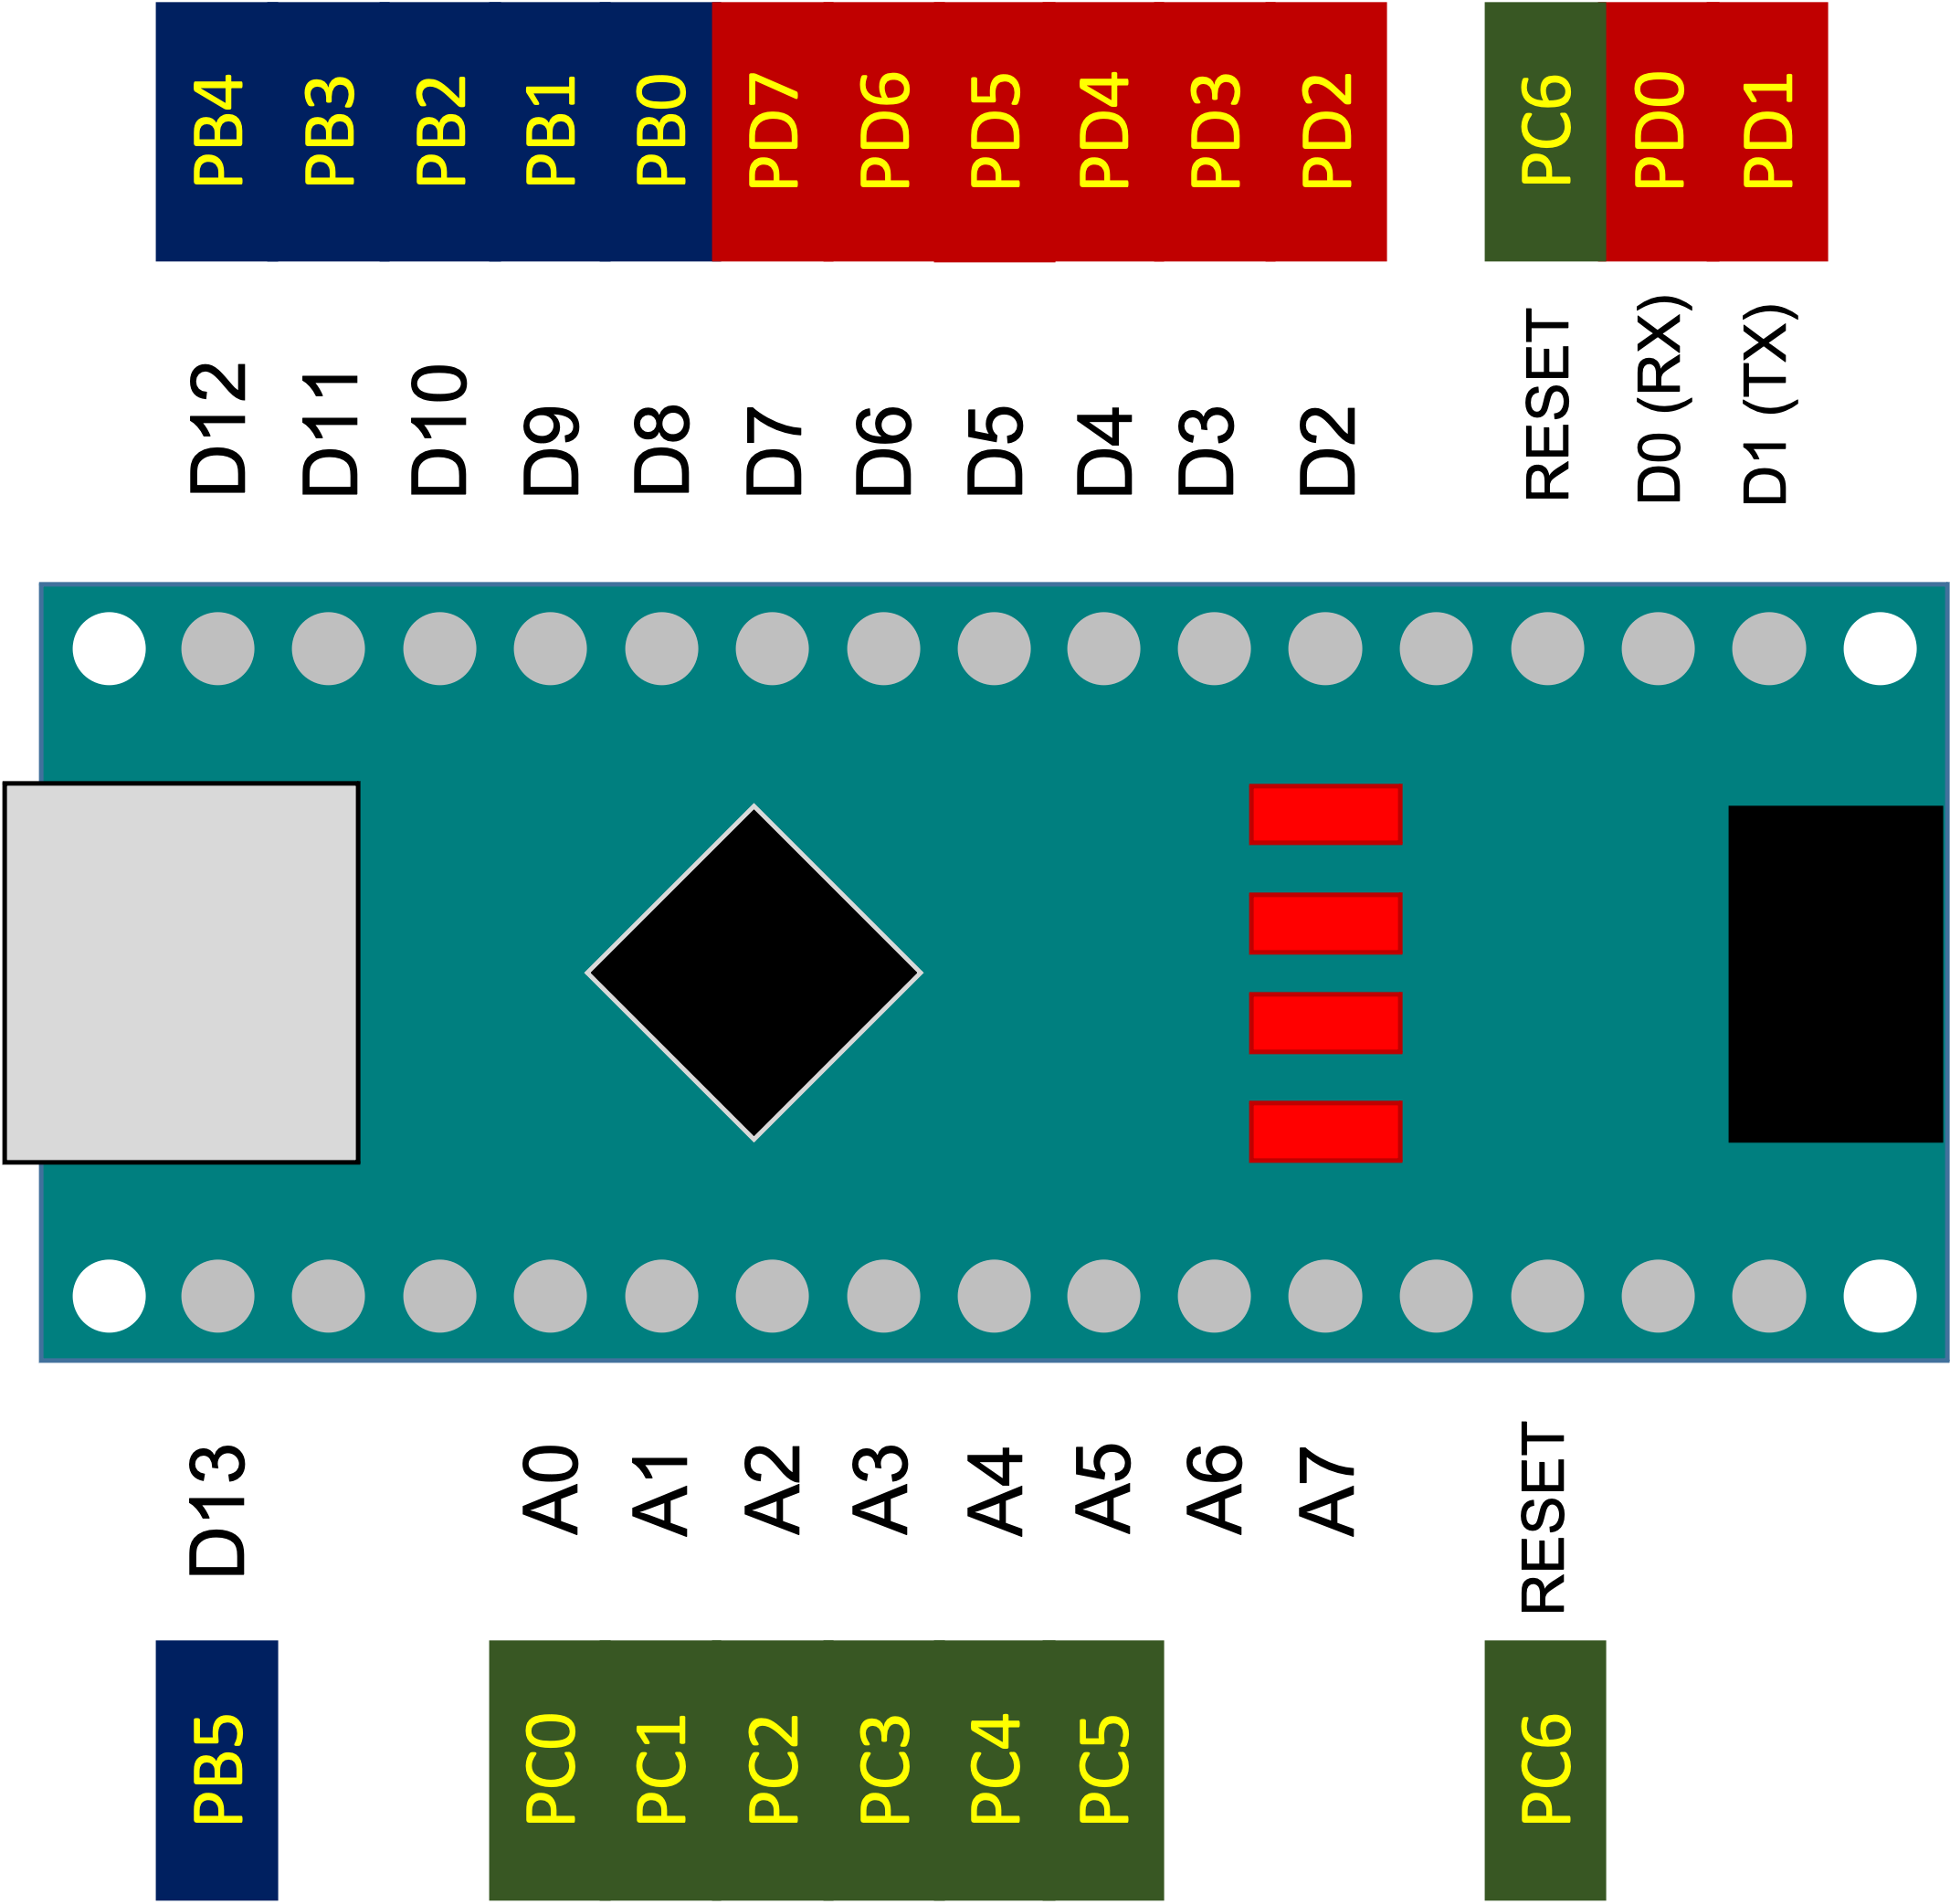
\includegraphics[width=10cm]{NanoPinMapping}
    \caption{Mapping of \nano\ pins to ATmega328P input/output ports. \tiny Diagram by Bohn \label{fig:NanoPinMapping}}
\end{figure}

Figure~\ref{fig:NanoPinMapping} shows which bit in which port corresponds to
each \nano\ pin. For example, pin \texttt{D10} is labeled ``PB2'' indicating
that it is part of port B and uses bit 2 in each of port B's registers. If
\texttt{D10} were an output pin, then we could set the pin's logic level to
high or low by assigning a 1 or 0, respectively, to \texttt{PORTB}'s bit 2.
On the other hand, if \texttt{D10} were an input pin, then we could determine
the pin's logic level by using a bitmask to examine \texttt{PORTB}'s bit 2.

\subsubsection{Accessing I/O Registers in Memory Address Space}

The header file \textit{cowpi.h} provides data structures to access the
memory-mapped I/O registers in a more readable form. For example, the
\lstinline{cowpi_ioPortRegisters} structure eliminates the need to remember
which I/O port registers are used for output to peripherals and which are used
for input from peripherals.

\lstinputlisting[linerange=168-172]{../starter-code/PollingLab/cowpi.h}

The \nano's three I/O ports are placed contiguously in the memory address space,
which will allow us to create a pointer to the lowest-addressed port and then
treat that pointer as an array of I/O ports. Some named constants that we can
use to index that array further eliminate the need to remember which port
corresponds to each \nano\ pin.

\lstinputlisting[linerange=164-166]{../starter-code/PollingLab/cowpi.h}

Finally, there is a constant pointer, \lstinline{cowpi_IObase} that holds the
memory address that is the start of ATmega328P's memory-mapped input/output
register bank, and a comment reminding us that the external pins' input/output
registers start 3 bytes above \lstinline{cowpi_IObase} (which is also
information we can get from Figure~\ref{fig:IoPortRegisters}).

\lstinputlisting[linerange=21-21]{../starter-code/PollingLab/cowpi.h}
\lstinputlisting[linerange=119-125, breaklines=true,
  postbreak=\mbox{\textcolor{red}{$\hookrightarrow$}\space}]{../starter-code/PollingLab/cowpi.h}

On line 17 of \textit{PollingLab.ino}, there is a global variable,
\lstinline{ioPorts} that will serve as our array of I/O ports.

    \begin{itemize}
    \item On line 50 of \textit{PollingLab.ino}, find this line in
        \function{setup()}: \lstinline{// ioPorts = ...}
    \item Remove the comment mark and ellipses, and assign to
        \lstinline{ioPorts} the address 3 bytes above \lstinline{IObase}; you
        will need to cast the resulting address to
        \lstinline{(cowpi_ioPortRegisters *)}.
    \end{itemize}

Index the \lstinline{cowpi_ioPortRegisters} array using the \lstinline{D8_D13},
\lstinline{A0_A5}, and \lstinline{D0_D7} named constants. Each element of the
array has an \lstinline{.input} field to read logic levels from peripherals and
a \lstinline{.output} field to assign logic levels for peripherals (as well as
a \lstinline{.direction} field that you won't use).

As you'll notice in Figure~\ref{fig:NanoPinMapping}, the lower-numbered pins
are their registers' less-significant bits (and thus are the less-significant
bits of the \lstinline{cowpi_ioPortRegisters}' fields), and the higher-numbered
pins are the more-significant bits. Continuing with our earlier example, if pin
\texttt{D10} were an input pin, then it would correspond with bit 2 of
\lstinline{ioPorts[D8_D13].input}. If pin \texttt{D10} were an output pin, then
it would correspond with bit 2 of \lstinline{ioPorts[D8_D13].output} (having the
third-lowest number in the range $13..8$, \texttt{D10} corresponds with the
third-least-significant bit).

To read the logic level of a specific pin or pins, apply a bitmask to the
appropriate array element's \lstinline{.input} field so that the resulting
bitfield preserves the bit(s) you're interested in and has 0s in the remaining
bits. To set the logic level of a specific pin or pins, apply the
read-modify-write pattern to the appropriate array element's
\lstinline{.output} field to set the value of the bit(s) you're interested in
and preserve the values of the remaining bit(s).

\subsubsection{Reading Polling Code}

The starter code includes a \function{testSimpleIO()} function. If you upload
\textit{PollingLab.ino} to your \nano, you will see on the Serial Monitor a
message whenever you press a button or toggle a switch. The external LED will
also light up whenever both switches are in the right position (if the room is
bright, you may have to shade the LED with your hand to see that it has
illuminated).

Recall that the left switch is connected to pin \texttt{A4} and the right
switch is connected to pin \texttt{A5}. Recall also that the left pushbutton is
connected to pin \texttt{D8} and the right pushbutton is connected to pin
\texttt{D9}. Notice that every time the \function{loop()} function iterates,
the pushbuttons' (pins \texttt{D8} \& \texttt{D9}) and switches' (pins
\texttt{A4} \& \texttt{A5}) logic values are checked, to determine if they have
taken on a value that we're interested in; that is, the code \textit{polls} the
input pins.

You may notice the code comparing \lstinline{now} with the time a button or
switch was last used and acting only if at least
\lstinline{BUTTON_NO_REPEAT_TIME} (500) or \lstinline{DEBOUNCE_TIME} (20)
milliseconds have passed. This serves two purposes.
\begin{description}
\item [Debouncing] Mechanical buttons and switches demonstrate a phenomenon
    called \textit{switch bounce}. This causes voltage to fluctuate for
    hundreds of microseconds when the contacts close or open. When this
    fluctuation is in the indeterminate region between the logical low and high
    thresholds, it can cause the logic level to ``bounce'' back-and-forth
    between high and low until settling into the final, correct logic level.
    This causes the digital circuitry or software to ``see'' multiple
    triggering events. \\
    \begin{itemize}
    \item The traditional way to debounce is to introduce a simple low-pass
    filter using a resistor and a capacitor. Hardware design can be
    simplified by solving a hardware problem with software, and so you will
    often see hobby projects with ``debouncing code'' such as
    \lstinline{delay(2);} that pauses execution between detecting the first
    change of the button's or switch's position and acting upon it for 2ms,
    ample time for switch bounce to stabilize. The problem (beyond
    \function{delay()} being disallowed in this lab) is that
    2,000µs is a long time to leave your system completely non-responsive.
    \item The solution used here allows your system to continue to respond to
    other external events. For example, you can press both buttons at very
    nearly the same time (or, unlikely, at the exact same time) and the
    software will react to both immediately.
    \end{itemize}
\item [Detecting single presses] If we did nothing, then when we pressed a
    button, the code that detects the button press would see the low logic
    value every time \function{loop()} iterated, causing the message to print
    repeatedly until we lifted our finger. The solution used here allows a
    momentary press of a button to be treated as a single event but also allows
    the user to continue to hold the button down and have the software
    recognize that the user has been holding it down longer. (In this
    particular case, ignoring the button for a half-second also provides for
    software debouncing.)
\end{description}

\subsubsection{Replacing Disallowed Function Calls}

The \function{testSimpleIO()} function uses \function{digitalRead()} and
\function{digitalWrite()}, two functions that are part of the Arudino core that
you cannot use in this lab. You need to remove these functions.

    \begin{itemize}
    \item Use the \lstinline{ioPorts} array to read from \texttt{A4},
        \texttt{A5}, \texttt{D8}, and \texttt{D9} instead of using
        \function{digitalRead()}. Confirm that \function{testSimpleIO()}
        functions the same.
    \item Now use the \lstinline{ioPorts} array to write to \texttt{D12}
        instead of using \function{digitalWrite()}. Confirm that
        \function{testSimpleIO()} functions the same.
    \end{itemize}

\subsection{Matrix Keypad}

The matrix keypad has sixteen buttons but connects only to eight pins. Instead
of reading the button presses directly, we scan the matrix to determine
which row and which column the pressed button is in. We do this by setting
logic levels on the rows and reading logic levels on the columns.

\begin{figure}
    \centering
    \subfloat[Front of matrix keypad.] {
        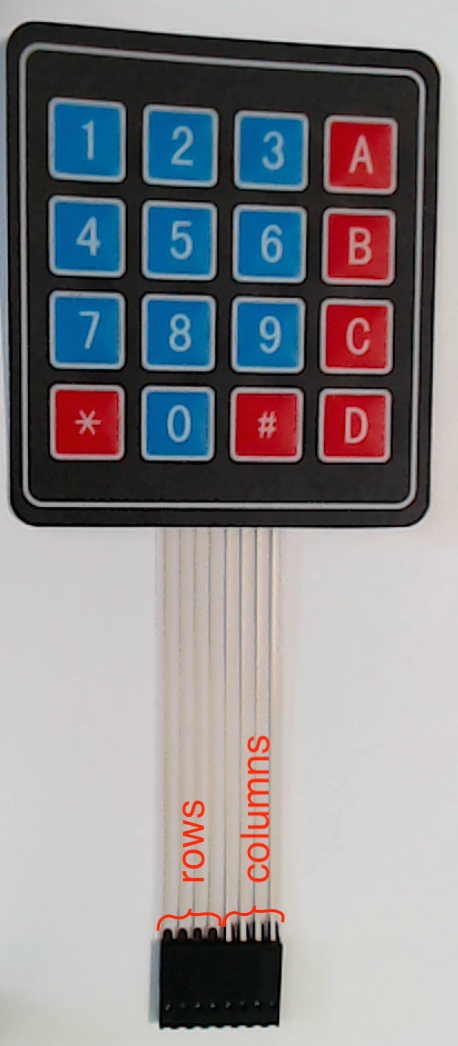
\includegraphics[height=8cm]{keypad-annotated}
    }
    \hfil
    \subfloat[Keypad's underlying contact matrix.] {
        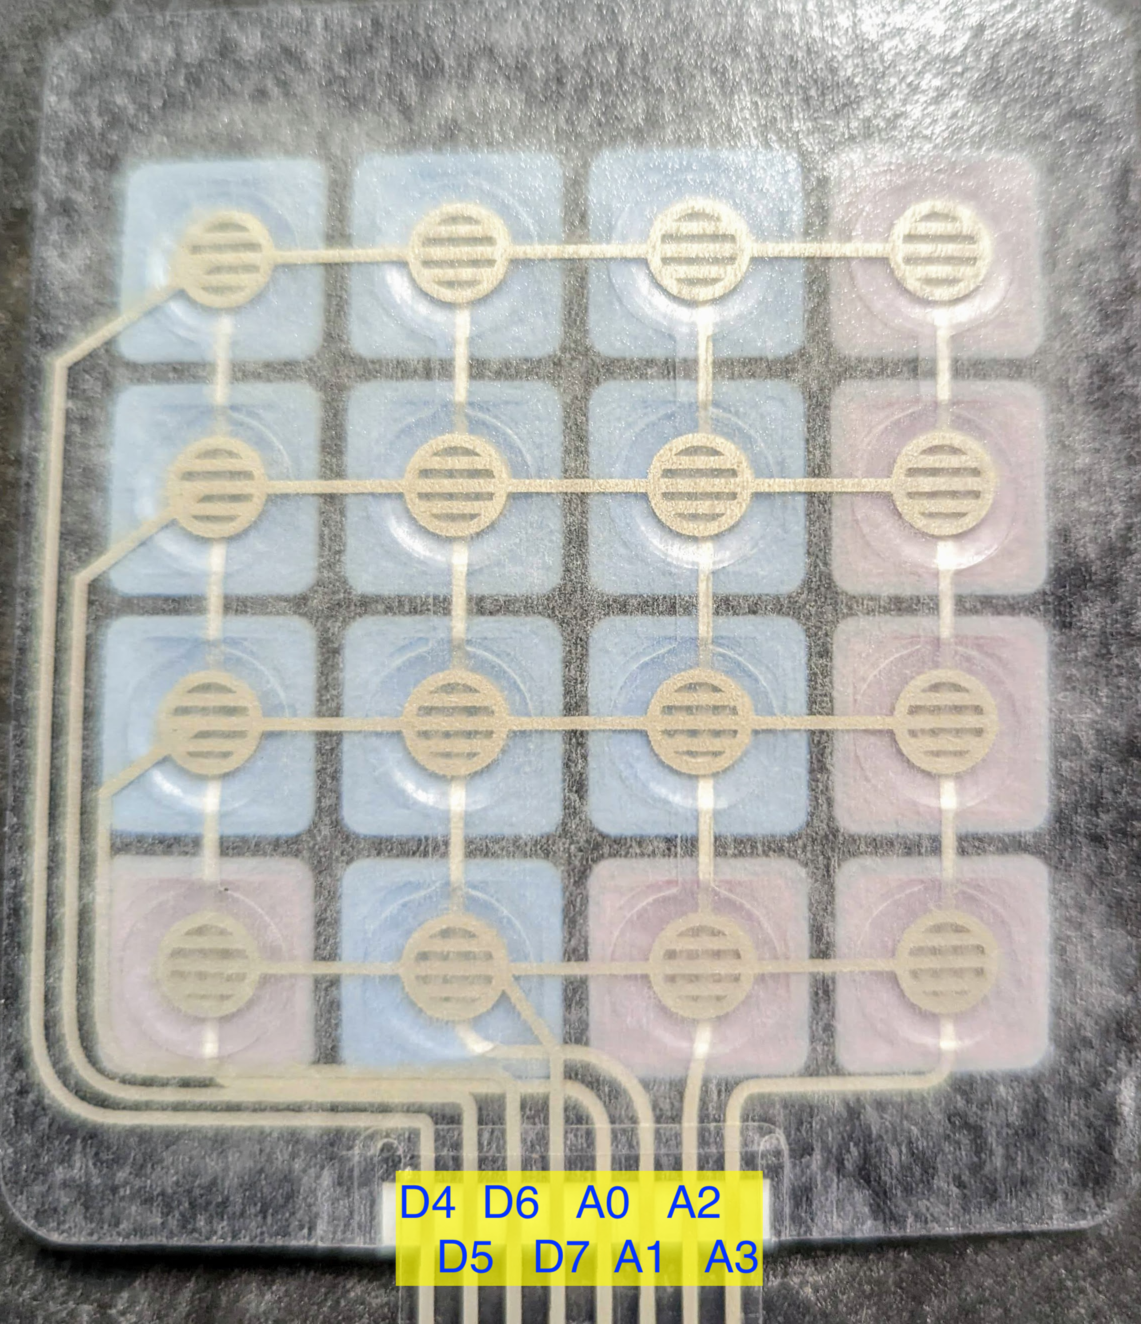
\includegraphics[height=8cm]{keypad-matrix}
    }
    \caption{The numeric keypad's header has four row pins and four column pins. \tiny Photographs and annotations by Bohn \label{fig:keypad-annotated}}
\end{figure}

    \begin{itemize}
    \item Recall that \texttt{row1} is connected to \texttt{D4}, \texttt{row4}
        pin to \texttt{D5}, \texttt{row7} to \texttt{D6}, and \texttt{row*} to
        \texttt{D7}.
    \item Recall that \texttt{column1} is connected to \texttt{A0},
        \texttt{column2} pin to \texttt{A1}, \texttt{column3} to \texttt{A2},
        and \texttt{columnA} to \texttt{A3}.
    \end{itemize}

\subsubsection{Scanning the Keypad}

There are a few options for obtaining the value corresponding to a key that is
pressed on the keypad. The most efficient for a simple application such as the
Number Building Tool is to use a lookup table. Starting on line 32 of
\textit{PollingLab.ino} you will find a 2-dimensional array that will serve as
the lookup table.
\lstinputlisting[linerange=29-40]{../starter-code/PollingLab/PollingLab.ino}
The element \lstinline{keys[0][0]} will correspond to the
\texttt{1} key; \lstinline{keys[0][3]} will correspond to the \texttt{A} key;
\lstinline{keys[3][0]} will correspond to the \texttt{*} key; and
\lstinline{keys[3][3]} will correspond to the \texttt{D} key.

We want the numerals \texttt{0}-\texttt{9} to produce their respective decimal
(and hexadecimal) values. We want \texttt{A}-\texttt{D} to produce their
respective hexadecimal values. We want \texttt{\#} to produce the hexadecimal
value 0xE, and we want \texttt{*} to produce the hexadecimal value 0xF.

    \begin{itemize}
    \item Populate \lstinline{keys}' nested array initializer so that the
        lookup table will produce the correct value for each row/column
        combination.
    \end{itemize}

The first step in reading a value from the keypad is determining whether a key
has been pressed. The \function{cowpi_setup} macro configured pins
\texttt{A0}-\texttt{A3} (connected to the columns) as input pins that pull
their logic values high when nothing forces them low. It also configured pins
\texttt{D4}-\texttt{D7} (connected to the rows) as output pins that initially
hold the value 0.

If no key has been pressed, then the column pins \texttt{A0}-\texttt{A3} will
all have the value 1 because nothing is pulling their logic values low. When a
button is pressed, the button's column will be electrically connected to the
button's row. Since the row pins \texttt{D4}-\texttt{D7} the value 0, this
will cause the button's column pin to take on the value 0. Thus, checking
whether \textit{any} button has been pressed can be accomplished by polling
pins \texttt{A0}-\texttt{A3} to determine if each holds the value 1 or if at
least one of them holds the value 0.

    \begin{itemize}
    \item Find the \lstinline{if} block starging on line 56 in
        \textit{PollingLab.ino}. Un-comment this \lstinline{if} block.
        \lstinputlisting[linerange=59-68]{../starter-code/PollingLab/PollingLab.ino}
    \item Replace the \lstinline{...} on line 56 with a conditional expression
        that evaluates to \texttt{true} whenever at least one of the column
        pins holds the value 0.
    \end{itemize}

Now locate \function{getKeyPressed()}.
\lstinputlisting[linerange=71-79]{../starter-code/PollingLab/PollingLab.ino}

    \begin{itemize}
    \item Inside the \lstinline{if} block, add a \lstinline{for} loop that
        iterates over the four rows.
    \item At the start of the loop body, set each row pin to output 1, except
        that the pin corresponding to the current iteration's row should output
        0. For example, in the first iteration, you want \texttt{D5},
        \texttt{D6}, and \texttt{D7} to output a 1 but \texttt{D4} to output a
        0. You will probably find it easier to do this in two lines, first
        setting \textit{all} of the row pins to 1 and then setting the current
        iteration's row pin to 0.
    \item Poll the column pins. If all column pins are still 1, then the key
        being pressed is not in the current iteration's row. On the other
        hand\dots
    \item If one of the column pins is 0, then the key being pressed is in the
        current iteration's row. If this is the case, then determine which
        column the key is in based on which column pin is has the value 0.
    \item Knowing the key's row and column, use the lookup table to assign the correct value to the variable \lstinline{keyPressed}.
        \begin{itemize}
        \item In case you make a mistake when writing this code, you may wish
            to add error-handling code to make sure you do not make an
            assignment to \lstinline{keysPressed} when you shouldn't have done
            so.
        \end{itemize}
    \item After the \lstinline{for} loop termintes, set the row pins back to 0.
    \end{itemize}

This design does \textit{not} handle the case of the user pressing multiple
keys simultaneously. Handling multiple simultaneous keypresses is a
considerably more-challenging problem.

\subsubsection{Testing Your Implementation}

If you implemented the keypad code correctly, then after you upload
\textit{PollingLab.ino} to your \nano, you will see on the Serial Monitor a
message with the key value whenever you press a key on the keypad. If it does
not, examine your code for errors. Adding debugging
\lstinline{Serial.print()}/\lstinline{Serial.println()} statements may help.

\subsection{7-Segment Display Module}

The 7-Segment Display Module consists of a
MAX7219\footnote{\url{https://datasheets.maximintegrated.com/en/ds/MAX7219-MAX7221.pdf}}
integrated circuit that acts as a peripheral using the SPI protocol and that
drives the eight 7-segment displays.

The \textit{Serial-Parallel Interface} (SPI) is a protocol that allows data to
be sent and received serially (over a single wire) that should be used in
parallel. This protocol is common enough that the ATmega328P microcontroller
used by the \nano\ implements the protocol in hardware (see chapter 18 of the
ATmega328P datasheet).

    \begin{quote}
    NOTE: The original SPI specification used the terms \textit{MOSI} and
    \textit{MISO} to describe its two modes, and alternately used \textit{SS}
    and \textit{CS} to describe the signal that a device should listen for
    input. The preferred terminology now is \textit{COPI} (Controller Output,
    Peripheral Input), \textit{CIPO} (Controller Input, Peripheral Output) to
    describe the modes in devices that can use either mode (such as the \nano),
    \textit{SDO} and \textit{SDI} to describe the modes in devices that can
    only use one mode (the display module uses SDI), and \textit{CS} (Chip
    Select) exclusively to describe the signal indicating that a device should
    listen for input.

    We will use the preferred terminology; however, legacy documentation --
    including the ATmega328P and MAX7219 datasheets -- still use the original
    terminology.
    \end{quote}

The MAX7219 receives the serial data into a shift register and then latches the
shift register's bits in parallel into one of eight memory locations or one of
five control registers. The \function{cowpi_setup} macro takes care of
configuring the MAX7219's control registers. Your task will be to write the
code that sends data to the display module.

Each of the eight memory locations in the MAX7219 each correspond to one of the
eight digits. The least-significant digit has the address 1, and the most-
significant digit has the address 8. The bit pattern in each of these addresses
indicates which LEDs in the 7-segment display should be illuminated (see
Figure~\ref{fig:SevenSegment}).

\begin{figure}
    \centering
    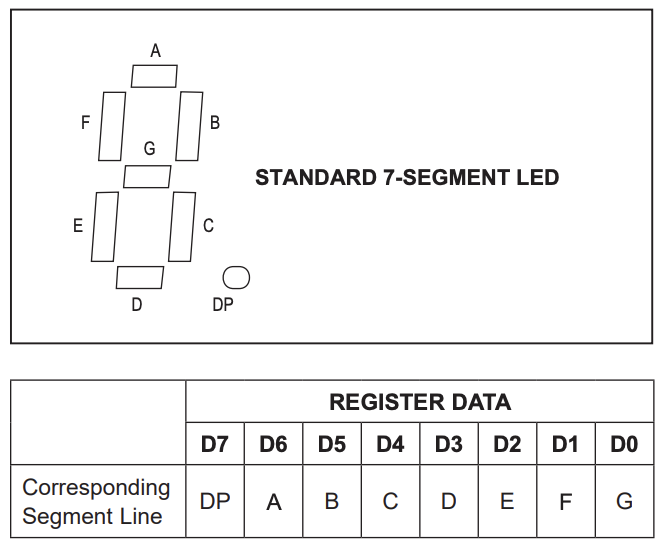
\includegraphics[width=10cm]{SevenSegment}
    \caption{Mapping of bits to 7-segment LEDs. \tiny Copied from MAX7219 Data Sheet, Table~6 \label{fig:SevenSegment}}
\end{figure}

Seven-segment displays are so-named because (not including the decimal point)
there are seven segments that can be activated/deactivated in combinations to
form the ten decimal numerals (and, with a little imagination, most of the
letters in the Latin alphabet). In the case of our display module, the segments
are LEDs; you might also see segmented displays using LCDs or flip panels.

\subsubsection{ATmega328P SPI Registers}

The ATmega328P uses three registers for SPI, \texttt{SPCR} which is used to
configure the SPI hardware, \texttt{SPSR} which is used to indicate the status
of a data transfer, and \texttt{SPDR} which is used to transfer data to and from
an SPI peripheral device (see Table~\ref{table:SPIregisters}).

The \function{cowpi_setup} macro enables SPI by setting the \texttt{SPE} bit to
1, sets the \nano\ as the controller by setting the Controller (née MSTR) bit
to 1, and sets the SPI clock at 1MHz by setting the SPR1 and SPR0 bits to 01.
All remaining bits in \texttt{SPCR} were set to 0.

\begin{table}
\centering \small
\begin{tabular}{|r||c|c|c|c|c|c|c|c||}
    \hline
    Bit                         & \textbf{7}    & \textbf{6}    & \textbf{5}    & \textbf{4}    & \textbf{3}    & \textbf{2}    & \textbf{1}    & \textbf{0}    \\ \cline{2-9} \cline{2-9}
    \textbf{SPDR} 0x2E (0x4E)   & MSB           & \dots         & \dots         & \dots         & \dots         & \dots         & \dots         & LSB           \\
    \textbf{SPSR} 0x2D (0x4D)   & SPIF          & WCOL          & not used      & not used      & not used      & not used      & not used      & SPI2X         \\
    \textbf{SPCR} 0x2C (0x4C)   & SPIE          & SPE           & DORD          & Controller    & CPOL          & CPHA          & SPR1          & SPR0          \\ \hline
\end{tabular}
\caption{SPI Data, Status, and Control Registers. \tiny Adapted from ATmega382P Data Sheet, §18.5. \label{table:SPIregisters}}
\end{table}

\subsubsection{Accessing SPI Registers in Memory Address Space}

The \lstinline{cowpi_spiRegisters} has three fields: \lstinline{control},
\lstinline{status}, and \lstinline{data}, corresponding to the \texttt{SPCR},
\texttt{SPSR}, and \texttt{SPDR} registers, respectively.

\lstinputlisting[linerange=174-178]{../starter-code/PollingLab/cowpi.h}

There is a global variable on line 18 of \textit{PollingLab.ino},
\lstinline{spi}, that we will use to access the SPI registers. If you look in
\textit{cowpi.h}, you will see a comment noting that the SPI registers start
0x2C bytes above \lstinline{cowpi_IObase}.

\lstinputlisting[linerange={119-123,135-136}]{../starter-code/PollingLab/cowpi.h}

    \begin{itemize}
    \item On line 51 of \textit{PollingLab.ino}, find this line in
        \function{setup}: \lstinline{// spi = ...}
    \item Remove the comment mark and ellipses, and assign to \lstinline{spi}
        the address 0x2C bytes above \lstinline{cowpi_IObase}; you will need to
        cast the resulting address to \lstinline{(cowpi_ioPortRegisters *)}.
    \end{itemize}

\subsubsection{Displaying Values}

We will use a lookup table to determine the bit patterns that need to be sent
to the display module. Starting on line 43 of \textit{PollingLab.ino} you will
find a 1-dimensional array that will serve as the lookup table.
\lstinputlisting[linerange=42-48]{../starter-code/PollingLab/PollingLab.ino}
The element \lstinline{sevenSegments[0]} will contain the bit pattern for the
numeral {\dviiseg 0},  \lstinline{sevenSegments[1]} will contain the bit
pattern for the numeral {\dviiseg 1}, and so on through
\lstinline{sevenSegments[15]} which will contain the bit pattern for the hex
numeral {\dviiseg F}. For reference, Figure~\ref{fig:SevenSegmentNumerals}
shows the desired segments to be activated for each of the sixteen numerals.
(Clearing a digit is achieved by sending 0x00 to that digit's corresponding
memory address, deactivating all segments for that digit. You do not need to
include this in the lookup table.)

\begin{figure}
    \centering
    {\dviiseg \huge 0123456789ABCDEF \\ \vspace{0.1cm}
                   8888888888888888}
    \caption{Segments to be activated for the sixteen numerals. The first row shows the segments to be activated; the second row shows all segments to more clearly show which segment is which. \label{fig:SevenSegmentNumerals}}
\end{figure}

In \function{displayData()}:
    \begin{itemize}
    \item Use the \lstinline{ioPorts} array to set \texttt{D10} to 0, instructing the display module to listen for data from the \nano.
    \item The MAX7219 expects the address to be sent before the value. Use the
        \lstinline{spi} struct's \lstinline{.data} field to place
        \lstinline{address} in the SPI Data Register.
    \item You should not place any new data into the SPI Data Register until
        the previous data has been sent; the \texttt{SPIF} bit in the SPI
        Status Register is a 0 when data is being sent and is a 1 when the data
        has been sent. Write a \lstinline{while} loop that does nothing except
        continue to iterate while the \texttt{SPIF} bit is a 0 (use the
        \lstinline{spi} struct's \lstinline{.status} field to poll the SPI
        Status Register).
    \item Now use the \lstinline{spi} struct to place \lstinline{value} in the
        SPI Data Register.
    \item Write another \lstinline{while} loop that does nothing except
        continue to iterate while the \texttt{SPIF} bit is a 0.
    \item Use the \lstinline{ioPorts} array to set \texttt{D10} to 1,
        instructing the display module to latch the data into its memory.
    \end{itemize}

\subsubsection{Testing Your Implementation}

On line 61 of \textit{PollingLab.ino}, find this line in \function{loop}: \\
\lstinline{// displayData(1, sevenSegments[keypress]);}. If you correctly
implemented the keypad code and the display code then any key you press on the
matrix keypad will display in the least-significant digit of the seven-segment
display module. If it does not, examine your code for errors. Adding debugging
\lstinline{Serial.print()}/\lstinline{Serial.println()} statements may help.

\subsection{Completing Demonstration Mode}

Most of the code for Demonstration Mode is now complete.

    \begin{itemize}
    \item Either remove the call to \function{testSimpleIO()} in
        \function{loop()} or remove the line in \function{testSimpleIO()} that
        causes the external LED to illuminate, since this is \textit{not} the
        behavior we want for the external LED.
    \item Add code to cause the external LED to illuminate when a key on the
        keypad is pressed and to deluminate 500ms later.
    \item Add code so that demonstration mode only executes when the left
        switch is in the left position.
    \item Add code so that when the right switch is in the right position, only
        decimal numerals (\textit{0-9}) are displayed.
    \item Add code so that when the user presses the right pushbutton, all
        digits on the display module are cleared.
    \end{itemize}

\section{Implementing Building Mode} \label{sec:BuildingMode}

When the system is not in demonstration mode, it is in building mode.

The best way to tackle building mode is to break it into bite-sized
subproblems. Start by implementing the code to build the value in accordance
with requirement~\ref{spec:BuildingValue}. Here are some recommendations:
    \begin{itemize}
    \item If you are running short on time, pay attention to the rubric to
        determine which requirements you should prioritize to maximize your
        score
    \item Start without considering the negation button.
    \item Start without worrying about handling values that are too big.
    \item Keep an array of the bit patterns to be displayed separate from the
        actual value being built.
        \begin{itemize}
        \item When a key is pressed, update both the value being built, the
        array of display bit patterns, and the actual display. The array can be
        updated simply by moving existing bit patterns into other positions in
        the array.
        \item This is a tradeoff -- maintaining both the value being built
        and a ``display buffer'' will require 8 extra bytes of your limited
        RAM, but your program will run faster (and you shouldn't need so much
        RAM that 8 bytes more or less will make a difference).
        \item If you maintain only the value being built and recalculate the BCD
        representation of a value every time a key is pressed in the decimal
        number base, this may become a performance bottleneck since division
        (and modulo) is not implemented in hardware, \textit{and} even the
        (8-bit) hardware-implemented addition/subtraction/multiplication will
        require several processor cycles for 32-bit arithmetic on the value.
        \item Some students in the past maintained only the ``display buffer''
        and recalculated the value being built after each keypress by applying
        a decimal (or hexadecimal) weighted-sum of the individual digits. This
        works but requires seven multiplications and seven additions.
        \textit{Updating} the value being built only requires one
        multiplication and one addition.
        \item Don't forget to print the value being built to the Serial Monitor.
        \end{itemize}
    \item Conveniently, you can also use the code to update the display array
        to detect when you need to display {\dviiseg too big} instead of making
        comparisons to the value being built.
    \end{itemize}

\begin{figure}
    \centering
    {\dviiseg \huge \begin{tabular}{r} too big \\
                                      88888888 \\
                                         % error
                                    \end{tabular}}
    \caption{Segments to be activated for error messages.
        % The first and third rows show the segments to be activated;.
        The first row shows the segments to be activated;
        the second row shows all segments to more clearly show which segment is
        which. \label{fig:SevenSegmentError}}
\end{figure}

Now that you have that code working, add code to negate the value whenever the
left pushbutton is pressed. It is possible to quickly update the display array
without using any arithmetic other than negating the value (how this is done
differs between the decimal and hexadecimal number bases), but if you need to
re-calculate the display array that is fine. Don't forget to update the actual
display, too.

Finally, remove any debugging
\lstinline{Serial.print()}/\lstinline{Serial.println()} statements so that when
in builder mode, only the value being built is printed to the Serial Montior.

\section*{Turn-in and Grading}

When you have completed this assignment, upload \textit{PollingLab.ino} to
\filesubmission.

This assignment is worth 40 points. \\

Rubric:
\begin{description}
\rubricitem{8}{Simple input/output functions correctly. (3 points for switches; 3 points for pushbuttons; 2 points for LED)}
\rubricitem{10}{Matrix keypad functions correctly.}
\rubricitem{8}{7-Segment Display Module functions correctly.}
\rubricitem{1}{System is in demonstration mode only when left switch is in left position and builder mode when the left switch is in the right position.}
\rubricitem{1}{External LED illuminates when key is pressed and deluminates 500ms later if in demonstration mode. (This behavior is unspecified when in building mode.)}
\rubricitem{2}{When in demonstration  mode, the numeral corresponding to the key pressed is displayed in the least-significant digit on the Display Module, in accordance with requirements~\ref{spec:decimalExplained}, \ref{spec:hexadecimalExplained}, and \ref{spec:demonstrationKeyPress}. (1 point for decimal number base; 1 point for hexadecimal number base)}
\rubricitem{1}{When in demonstration mode, the right pushbutton clears the display.}
\rubricitem{2}{Builds a value consistent with requirements~\ref{spec:decimalExplained} and \ref{spec:BuildingValue} when in building mode and using the decimal number base. (\textonehalf\ point for each of: printing correct positive values, printing correct negative values, displaying correct positive values, displaying correct negative values)}
\rubricitem{2}{Builds a value consistent with requirements~\ref{spec:hexadecimalExplained} and \ref{spec:BuildingValue} when in building mode and using the hexadecimal number base. (\textonehalf\ point for each of: printing correct positive values, printing correct negative values, displaying correct positive values, displaying correct negative values)}
\rubricitem{1}{Negates value in the decimal number base when left pushbutton is pressed while in building mode. (\textonehalf\ point for each of: printing and displaying correct positive values, printing and displaying correct negative values)}
\rubricitem{1}{Negates value in the hexadecimal number base when left pushbutton is pressed while in building mode. (\textonehalf\ point for each of: storing and displaying correct positive values, storing and displaying correct negative values)}
\rubricitem{2}{Detects and displays correct message when the number being built is too big. (\textonequarter\ point for detecting too-big numbers for each of: positive decimal numbers, negative decimal numbers, positive hexadecimal numbers, negative hexadecimal numbers; \textonequarter\ point for no false detections among each of: decimal numbers, hexadecimal numbers; \textonehalf\ point for printing the correct message)}
\rubricitem{1}{When in building mode the right pushbutton clears all digits on the Display Module except the least-significant digit, which displays {\dviiseg 0}.}
\bonusitem{2}{Get assignment checked-off by TA or professor during office hours before it is due. (You cannot get both bonuses.)}
\bonusitem{1}{Get assignment checked-off by TA at \textit{start} of your scheduled lab immediately after it is due. (Your code must be uploaded to \filesubmission\ \textit{before} it is due. You cannot get both bonuses.)}
\item[Penalties]
\penaltyitem{8}{Simple input/output configuration and test function relies on code that violates the constraints in Section~\ref{sec:Constraints}.}
\penaltyitem{10}{Obtaining values from matrix keypad relies on code that violates the constraints in Section~\ref{sec:Constraints}.}
\penaltyitem{8}{Sending values to the 7-segment display module relies on code that violates the constraints in Section~\ref{sec:Constraints}.}
\penaltyitem{5}{Code associated with demonstration mode (other than that covered in the first three penalty items) relies on code that violates the constraints in Section~\ref{sec:Constraints}.}
\penaltyitem{9}{Code associated with conversion mode (other than that covered in the first three penalty items) relies on code that violates the constraints in Section~\ref{sec:Constraints}.}
\spaghetticodepenalties{1}
\end{description}

\section*{Epilogue}

Herb looks over your work. ``Hmm, yes. I think this is coming along nicely.
Let's run a few more tests.''

Archie storms into the room. ``We have \textit{got} to do something about
security! How's that doodad coming along? Because there's now a
 half-man/half-fly in the labs going on-and-on about Chaos Theory and how if we
 just give him a MacBook and a spaceship then he'll be able to get the Lord of
 Thunder to travel across the 8th Dimension. Is that thing just about ready?''

Herb shakes his head, ``No, not quite yet. It should be ready in about a week.''

\textit{To be continued...}

\newpage

\section*{Appendix: Lab Checkoff}

You are not required to have your assignment checked-off by a TA or the
professor. If you do not do so, then we will perform a functional check
ourselves. In the interest of making grading go faster, we are offering a small
bonus to get your assignment checked-off at the start of your scheduled lab
time immediately after it is due. Because checking off all students during lab
would take up most of the lab time, we are offering a slightly larger bonus if
you complete your assignment early and get it checked-off by a TA or the
professor during office hours.

\begin{description}
\item [] (\phantom{xxx}) Establish that the code you are demonstrating is the code
    you submitted to to \filesubmission.
    \begin{itemize}
    \item If you are getting checked-off during lab time, show the TA that the
        file was submitted before it was due.
    \item Download the file into your PollingLab directory. If necessary,
        rename it to \textit{PollingLab.ino}.
    \end{itemize}
\item [] (\phantom{xxx}) Upload \textit{PollingLab.ino} to your \nano.
\end{description}
\textbf{If you completed demonstration mode, jump ahead to
\textit{Demonstration Mode}.} Successfully completing demonstration
\textit{prima facie} shows that the I/O functions correctly.

\textbf{If you did not complete demonstration mode:}
\renewcommand{\labelenumi}{\Alph{enumi}.}
\begin{enumerate}
\item (\phantom{xxx}) Using \function{testSimpleIO()}, show on the Serial
    Monitor that the left and right button presses are detected. \\
    \textit{+1\textonehalf\ pushbutton presses detected} \\
    \textit{+1\textonehalf\ left and right pushbuttons are distinguished from
    each other}
\item (\phantom{xxx}) Using \function{testSimpleIO()}, show on the Serial
    Monitor that the left and right switches' position changes are detected. \\
    \textit{+1\textonehalf\ switch positions detected} \\
    \textit{+1\textonehalf\ left and right switches are distinguished from
    each other}
\item (\phantom{xxx}) Show that the external LED illuminates when it is
    supposed to (in a bright room, you may need to shade the LED with your
    hand). You can do this either by moving both switches to the right position
    (using the code in \function{testSimpleIO()}) or by showing the LED
    illuminate when you press a key on the matrix keypad (if you started
    working on demonstration mode). \\
    \textit{+2 LED works}
\item (\phantom{xxx}) Show on the Serial Monitor that key presses on the matrix
    keypad are correctly decoded. \\
    \textit{+10 keypad works}
\item (\phantom{xxx}) Show on the display module that values decoded from the
    matrix keypad are displayed as the correct characters. \\
    \textit{+8 display module works}
\end{enumerate}
\renewcommand{\labelenumi}{\arabic{enumi}.}
\begin{enumerate}
\item [] \textbf{\textit{Demonstration Mode}}
\item (\phantom{xxx}) Place both switches in the left position. The display
    module is initially blank.
\item(\phantom{xxx}) Press a number key on the matrix keypad. The corresponding
    character appears on the display module, and the external LED illuminates
    for approximately one-half of a second. \\
    \textit{+1 LED illumination} \\
    \textit{+2 LED works}
\item (\phantom{xxx}) Press a different number key on the matrix keypad.
    The corresponding character appears on the display module, and the external
    LED illuminates for approximately one-half of a second. \\
    \textit{+\textonehalf\ decimal numeral} \\
    \textit{+10 keypad works} \\
    \textit{+8 display module works}
\item (\phantom{xxx}) Press a letter key on the matrix keypad. The display
    module is unchanged. \\
    \textit{+\textonehalf\ letter rejected in decimal number base}
\item (\phantom{xxx}) Place the right switch in the right position. The display
    is unchanged.
\item (\phantom{xxx}) Press a letter key on the matrix keypad. The
    corresponding character appears on the display module, and the external LED
    illuminates for approximately one-half of a second. \\
    \textit{+1 hexadecimal numeral} \\
    \textit{+1\textonehalf\ switch positions detected}
\item (\phantom{xxx}) Press the right pushbutton. The display module blanks. \\
    \textit{+1 clear display} \\
    \textit{+1\textonehalf\ pushbutton presses detected}
\item (\phantom{xxx}) Press a key on the matrix keypad. The corresponding
    character appears on the display module, and the external LED illuminates
    for approximately one-half of a second. \\
    \textit{establishes that demonstration mode continues to work; if not then
    deduct half of the decimal/hexadecimal numeral points (if any)}
\item (\phantom{xxx}) Press the same key on the matrix keypad. The display
    module is unchanged (still displays the corresponding character), but the
    external LED still illuminates for approximately one-half of a second. \\
    \textit{establishes that the same key can be pressed twice with
    well-defined behavior; if the display changes then deduct half of the
    decimal/hexadecimal numeral points (if any); if the LED does not illuminate
    then deduct half of the ``LED illumination'' point (if any) but not the
    ``LED works'' points}
\item (\phantom{xxx}) Press the left pushbutton. Nothing happens. \\
    \textit{+1\textonehalf\ left and right pushbuttons are distinguished from
    each other}
\item[] \textbf{\textit{Demonstration Mode and Building Mode are Different}}
\item (\phantom{xxx}) Place the left switch in the right position. The display
    remains unchanged.
\item (\phantom{xxx}) Press the right pushbutton. The display shows \\
    {\dviiseg\phantom{0000000}0}\hspace{1cm}(additional leading 0s are allowed)
    \\ and the Serial Monitor shows \\
    {\dviiseg\phantom{00000000}}\hspace{1cm}\texttt{0} \\
    \textit{+1 left switch selects mode} \\
    \textit{+1\textonehalf\ left and right switches are distinguished from
    each other}
\item[] \textbf{\textit{Building Mode}}
\item (\phantom{xxx}) Place the right switch in the left position. The display
    remains unchanged.
\item (\phantom{xxx}) Press 2, then 3. \\
    {\dviiseg \phantom{0000000}2}\hspace{1cm}\texttt{2} \\
    {\dviiseg \phantom{000000}23}\hspace{1cm}\texttt{23}
\item (\phantom{xxx}) Press B. The display is unchanged. \\
    \textit{printing (+\textonehalf) \& displaying (+\textonehalf) positive decimal numbers}
\item (\phantom{xxx}) Press the left pushbutton, then 1. \\
    {\dviiseg \phantom{00000}-23}\hspace{1cm}\texttt{-23}\hspace{1cm}
    \textit{+\textonehalf\ negates decimal positive values} \\
    {\dviiseg \phantom{0000}-231}\hspace{1cm}\texttt{-231}\hspace{1cm}
    \textit{printing (+\textonehalf) \& displaying (+\textonehalf) negative decimal numbers}
\item (\phantom{xxx}) Press the left pushbutton, then 4. \\
    {\dviiseg \phantom{00000}231}\hspace{1cm}\texttt{231}\hspace{1cm}
    \textit{+\textonehalf\ negates decimal negative values} \\
    {\dviiseg \phantom{0000}2314}\hspace{1cm}\texttt{2314}\hspace{1cm}
    \textit{establishes that building mode continues to work}
\item (\phantom{xxx}) Press D. The display is unchanged. \\
    \textit{establishes that building mode continues to work; if building mode
    does not work after negation, deduct half of the printing/displaying
    decimal points (if any)}
\item (\phantom{xxx}) Press the right pushbutton, and place the right switch in
    the right position. \\
    {\dviiseg\phantom{0000000}0}\hspace{1cm}\texttt{0}\hspace{1cm}
    \textit{+1 display resets to 0}
\item(\phantom{xxx}) Press \#, then 7. \\
    {\dviiseg \phantom{0000000}E}\hspace{1cm}\texttt{E} \\
    {\dviiseg \phantom{000000}E7}\hspace{1cm}\texttt{E7}\hspace{1cm}
    \textit{printing (+\textonehalf) \& displaying (+\textonehalf) positive hex
    numbers}
\item (\phantom{xxx}) Press the left pushbutton. \\
    {\dviiseg FFFFFF19}\hspace{1cm}\texttt{FFFFFF19}\hspace{1cm}
    \textit{+\textonehalf\ negates hex positive values}
\item(\phantom{xxx}) Press 0, then A. \\
    {\dviiseg FFFFF190}\hspace{1cm}\texttt{FFFFF190} \\
    {\dviiseg FFFF190A}\hspace{1cm}\texttt{FFFF190A}\hspace{1cm}
    \textit{printing (+\textonehalf) \& displaying (+\textonehalf) negative hex
    numbers}
\item(\phantom{xxx}) Press the left pushbutton, then *. \\
    {\dviiseg \phantom{0000}E6F6}\hspace{1cm}\texttt{E6F6}\hspace{1cm}
    \textit{+\textonehalf\ negates hex negative values} \\
    {\dviiseg \phantom{000}E6F6F}\hspace{1cm}\texttt{E6F6F}\hspace{1cm}
    \textit{establishes that building mode continues to work}
\item(\phantom{xxx}) Press B, then C, then D, then 0. \\
    {\dviiseg \phantom{00}E6F6FB}\hspace{1cm}\texttt{E6F6FB} \\
    {\dviiseg \phantom{0}E6F6FBC}\hspace{1cm}\texttt{E6F6FBC} \\
    {\dviiseg           E6F6FBCD}\hspace{1cm}\texttt{E6F6FBCD}\hspace{1cm}
    \textit{no false detection - hex \#1} \\
    {\dviiseg \phantom{0}too big}\hspace{1cm}\texttt{too big}\hspace{1cm}
    \textit{too big - negative hex \#1}
\item (\phantom{xxx}) Press the right pushbutton; then press 1, then 2, then 3, then A, then B, then 6, then 5, then 4, then 7. \\
    {\dviiseg \phantom{0000000}0}\hspace{1cm}\texttt{0} \\
    {\dviiseg \phantom{0000000}1}\hspace{1cm}\texttt{1} \\
    {\dviiseg \phantom{000000}12}\hspace{1cm}\texttt{12} \\
    {\dviiseg \phantom{00000}123}\hspace{1cm}\texttt{123} \\
    {\dviiseg \phantom{0000}123A}\hspace{1cm}\texttt{123A} \\
    {\dviiseg \phantom{000}123AB}\hspace{1cm}\texttt{123AB} \\
    {\dviiseg \phantom{00}123AB6}\hspace{1cm}\texttt{123AB6} \\
    {\dviiseg \phantom{0}123AB65}\hspace{1cm}\texttt{123AB65} \\
    {\dviiseg           123AB654}\hspace{1cm}\texttt{123AB654}\hspace{1cm}
    \textit{no false detection - hex \#2} \\
    {\dviiseg \phantom{0}too big}\hspace{1cm}\texttt{too big}\hspace{1cm}
    \textit{+\textonequarter\ too big - positive hex}
\item (\phantom{xxx}) Press the right pushbutton; then push *, then 2, then 3, then A, then B, then 6, then 5, then 4, then 7. \\
    {\dviiseg \phantom{0000000}0}\hspace{1cm}\texttt{0} \\
    {\dviiseg \phantom{0000000}F}\hspace{1cm}\texttt{F} \\
    {\dviiseg \phantom{000000}F2}\hspace{1cm}\texttt{F2} \\
    {\dviiseg \phantom{00000}F23}\hspace{1cm}\texttt{F23} \\
    {\dviiseg \phantom{0000}F23A}\hspace{1cm}\texttt{F23A} \\
    {\dviiseg \phantom{000}F23AB}\hspace{1cm}\texttt{F23AB} \\
    {\dviiseg \phantom{00}F23AB6}\hspace{1cm}\texttt{F23AB6} \\
    {\dviiseg \phantom{0}F23AB65}\hspace{1cm}\texttt{F23AB65} \\
    {\dviiseg           F23AB654}\hspace{1cm}\texttt{F23AB654}\hspace{1cm}
    \textit{no false detection - hex \#3} \\
    {\dviiseg \phantom{0}too big}\hspace{1cm}\texttt{too big}\hspace{1cm}
    \textit{too big - negative hex \#2}
\item (\phantom{xxx}) Press the right pushbutton; then push *, then 9, then 3, then A, then B, then 6, then 5, then 4, then 7, then 8. \\
    {\dviiseg \phantom{0000000}0}\hspace{1cm}\texttt{0} \\
    {\dviiseg \phantom{0000000}F}\hspace{1cm}\texttt{F} \\
    {\dviiseg \phantom{000000}F9}\hspace{1cm}\texttt{F9} \\
    {\dviiseg \phantom{00000}F93}\hspace{1cm}\texttt{F93} \\
    {\dviiseg \phantom{0000}F93A}\hspace{1cm}\texttt{F93A} \\
    {\dviiseg \phantom{000}F93AB}\hspace{1cm}\texttt{F93AB} \\
    {\dviiseg \phantom{00}F93AB6}\hspace{1cm}\texttt{F93AB6} \\
    {\dviiseg \phantom{0}F93AB65}\hspace{1cm}\texttt{F93AB65} \\
    {\dviiseg           F93AB654}\hspace{1cm}\texttt{F93AB654} \\
    {\dviiseg           93AB6547}\hspace{1cm}\texttt{93AB6547}\hspace{1cm}
    \textit{no false detection - hex \#4} \\
    {\dviiseg \phantom{0}too big}\hspace{1cm}\texttt{too big}\hspace{1cm}
    \textit{too big - negative hex \#3} \\
    \textit{+\textonequarter\ for all three ``too bit - negative hex''} \\
    \textit{+\textonequarter\ for all four ``no false detection - hex''}
\item (\phantom{xxx}) Press the right pushbutton, and place the right switch in
    the left position. \\
    {\dviiseg \phantom{0000000}0}\hspace{1cm}\texttt{0}
\item (\phantom{xxx}) Press 5, then 6, then 7, then 8, then 9, then 0, then 1, then 2, then 3. \\
    {\dviiseg \phantom{0000000}5}\hspace{1cm}\texttt{5} \\
    {\dviiseg \phantom{000000}56}\hspace{1cm}\texttt{56} \\
    {\dviiseg \phantom{00000}567}\hspace{1cm}\texttt{567} \\
    {\dviiseg \phantom{0000}5678}\hspace{1cm}\texttt{5678} \\
    {\dviiseg \phantom{000}56789}\hspace{1cm}\texttt{56789} \\
    {\dviiseg \phantom{00}567890}\hspace{1cm}\texttt{567890} \\
    {\dviiseg \phantom{0}5678901}\hspace{1cm}\texttt{5678901} \\
    {\dviiseg           56789012}\hspace{1cm}\texttt{56789012}\hspace{1cm}
    \textit{no false detection - decimal \#1} \\
    {\dviiseg \phantom{0}too big}\hspace{1cm}\texttt{too big}\hspace{1cm}
    \textit{+\textonequarter\ too big - positive decimal}
\item (\phantom{xxx}) Press the right pushbutton; then press 3, then the left pushbutton, then 4, then 5, then 6, then 7, then 8, then 9, then 0. \\
    {\dviiseg \phantom{0000000}0}\hspace{1cm}\texttt{0} \\
    {\dviiseg \phantom{0000000}3}\hspace{1cm}\texttt{3} \\
    {\dviiseg \phantom{000000}-3}\hspace{1cm}\texttt{-3} \\
    {\dviiseg \phantom{00000}-34}\hspace{1cm}\texttt{-34} \\
    {\dviiseg \phantom{0000}-345}\hspace{1cm}\texttt{-345} \\
    {\dviiseg \phantom{000}-3456}\hspace{1cm}\texttt{-3456} \\
    {\dviiseg \phantom{00}-34567}\hspace{1cm}\texttt{-34567} \\
    {\dviiseg \phantom{0}-345678}\hspace{1cm}\texttt{-345678} \\
    {\dviiseg           -3456789}\hspace{1cm}\texttt{-3456789}\hspace{1cm}
    \textit{no false detection - decimal \#2} \\
    {\dviiseg \phantom{0}too big}\hspace{1cm}\texttt{too big}\hspace{1cm}
    \textit{+\textonequarter\ too big - negative decimal} \\
    \textit{+\textonequarter\ for both ``no false detection - decimal''} \\
    \textit{+\textonehalf\ if all ``too big'' displayed the correct message;
    +\textonequarter\ if all but one ``too big'' displayed the correct message}
\end{enumerate}

This concludes the demonstration of your system's functionality. The TAs will
later examine your code for violations of the assignment's constraints. If your
code looks like it is tailored for this checklist, the TAs may re-grade using a
different checklist\texttt{.}
\end{document}
